\documentclass[11pt]{article}

\usepackage[a4paper,margin=2.6cm]{geometry}
\usepackage[T1]{fontenc}
\usepackage[utf8]{inputenc}
\usepackage{lmodern}
\usepackage{microtype}
\usepackage{amsmath,amssymb}
\usepackage{booktabs}
\usepackage{graphicx}
\usepackage{xcolor}
\usepackage[font=small,labelfont=bf]{caption}
\usepackage{enumitem}
\definecolor{linkblue}{HTML}{1c5cab}
\usepackage[colorlinks=true,linkcolor=linkblue,citecolor=linkblue,urlcolor=linkblue]{hyperref}

\newcommand{\sillage}{\textsc{Sillage}}

\title{\bfseries Found Is Not Formulated:\\
A Gradient-Free Memory Meets LongMemEval}
\author{Abderrahmane Sghairi\\
\small Independent Researcher, Issoire, France\\
\small \texttt{sghairipro63@gmail.com}}
\date{August 2026\\[2pt]
\small DOI: \href{https://doi.org/10.5281/zenodo.ZZDOI7}{10.5281/zenodo.ZZDOI7}
\qquad Code: \href{https://github.com/riscoss63/sillage}{github.com/riscoss63/sillage}}

\begin{document}
\maketitle

\begin{abstract}
The companion paper of this series established six behavioral laws of the \sillage{} memory system on invented-fact instruments \cite{behavior}; this paper asks whether those laws survive contact with an external benchmark the system was never tuned on. We run LongMemEval \cite{longmemeval} --- 500 questions, each over $\sim$115k tokens of chat history --- through the tool's two voices, with deterministic, judge-free metrics and every prediction registered before each run. \textbf{The extractive voice} (the lexical index behind \texttt{sillage ask}; no model, no GPU) surfaces an evidence session in its top-3 passages for \textbf{92.6\%} of questions --- in 17 minutes on a desktop CPU for the entire benchmark --- while the gold answer string appears verbatim in those passages for only 29.6\%: a \textbf{63-point gap} between \emph{finding} and \emph{formulating} that decomposes exactly along question type (user facts 78\% formulated; multi-session aggregation 11\%; date arithmetic 10\%). \textbf{The generative voices} (Qwen3-0.6B, 43-question stratified sample, three arms per question) measure where formulation happens: memory alone answers 5\%; context alone 25\%; context \emph{plus} memory 25\% --- and not merely equal on average but \textbf{identical on all 40 scored questions}: the surprise gate prices in-window redundancy at exactly zero, so a 121k-token memory is perfectly neutral in the retrieval-augmented regime, question by question. Running the benchmark at all required removing ingestion's hidden tax: profiling shows two rank-1 outer products --- $\sim$50\,MB of memory traffic per token, all of it spent \emph{pricing} the memory rather than building it --- and applying the writes in 64-token GEMM blocks reaches \textbf{306 tokens/s} on the benchmark worker, $\times$43 over the shipped read path, with cold-store admissions, counts and masses exact by construction and every tolerance declared and tested. Eight predictions were registered: seven confirmed, one refuted and kept (evidence coverage is \emph{better} than predicted --- the deficit is formulation, not finding). These are retrieval-style and containment metrics, not judged QA accuracy; no number here is comparable to a leaderboard. What the benchmark shows is the laws holding out of distribution: \emph{the wake finds; the window speaks}.
\end{abstract}

\section{Introduction}

A memory system for frozen language models can be evaluated two ways: on instruments built to expose its mechanisms, or on benchmarks built by someone else. The six papers of this series did the first --- likelihood and recall on private corpora \cite{sillage,router,hier,fw}, cross-model transfer and exact speculative acceleration \cite{drafter}, and finally a behavioral anatomy on invented facts \cite{behavior} whose laws say precisely \emph{where} stored information does and does not become behavior. The obvious objection stands: instruments are ours. This paper takes the system, unchanged and untuned, to LongMemEval \cite{longmemeval}, a 500-question benchmark of long-term conversational memory whose haystacks ($\sim$115k tokens, $\sim$50 chat sessions per question) dwarf anything the tool was built on.

Two commitments shape the method. First, \emph{judge-free scoring}: LongMemEval's headline metric is QA accuracy judged by a large commercial model; we replace it with deterministic proxies --- evidence-session retrieval for the extractive voice, normalized answer-string containment for the generative voices --- that anyone can recompute from the committed JSONs. The cost is comparability (none of our numbers is a leaderboard number, and we never present them as one); the gain is that every figure in this paper is reproducible to the digit with no API key. Second, \emph{pre-registration}: as throughout the series, each arm's predictions --- including numeric falsification thresholds --- were written in the released log before the run, and the one prediction the data refuted is reported with the same prominence as the seven it confirmed.

\paragraph{Contributions.}
\begin{enumerate}[leftmargin=1.5em,itemsep=2pt]
\item \textbf{Found is not formulated, at benchmark scale} (\S\ref{sec:arme}): the tool's lexical index surfaces an evidence session in the top-3 for 92.6\% of 500 questions, in 17 minutes on a desktop CPU with no model, while strict answer presence is 29.6\% --- a 63-point gap that follows the formulation gradient predicted by the first law of \cite{behavior}.
\item \textbf{The memory is exactly neutral in the RAG regime} (\S\ref{sec:armg}): with evidence in the window, context+memory equals context-alone on \emph{every one} of 40 questions --- the behavioral, benchmark-scale face of the surprise gate's in-window pricing (law 6 of \cite{behavior}).
\item \textbf{Ingestion without the pricing tax} (\S\ref{sec:ingest}): a profile locates $\sim$86\% of per-token cost in two rank-1 outer products; applying writes in 64-token GEMM blocks yields $\times$43 throughput with an exactness contract (admissions, counts, masses, counters: identical; amplitudes and reservoir quantiles: bounded, declared, tested) --- the engineering artifact this benchmark forced, as speculative decoding was forced by \cite{drafter}.
\item \textbf{A pre-registered scorecard} (\S\ref{sec:laws}): eight predictions derived from the companion paper's laws, seven confirmed and one refuted; the refutation (evidence coverage better than predicted) sharpens the conclusion rather than weakening it.
\end{enumerate}

\section{Related work}

LongMemEval \cite{longmemeval} is the reference benchmark for long-term interactive memory; its own results show frontier long-context systems dropping $\sim$30\% accuracy as history grows, and its evaluation relies on an LLM judge. Judged accuracy and our deterministic proxies measure different things, and we keep the regimes strictly apart. The extractive voice descends from classical lexical retrieval \cite{bm25}; retrieval-augmented generation \cite{rag} is voice (b) of our design, with the twist that here the retriever and the memory are the same object read two ways. Behavioral evaluation of memory claims follows \cite{beyondppl}, whose insistence on probing \emph{use} rather than likelihood this series adopted in \cite{behavior}; the present paper is that program's external-validity stage. kNN-LM's likelihood-without-behavior gap \cite{khandelwal2020} is the ancestral observation behind our first law, and it reappears here at benchmark scale as the found/formulated gap.

\section{Benchmark, voices, and metrics}\label{sec:setup}

\textbf{Data.} LongMemEval-S \cite{longmemeval}: 500 questions over synthetic user--assistant chat histories ($\sim$115k tokens, median 50 sessions per question), in six types --- single-session (user, assistant, preference), knowledge-update, multi-session, temporal-reasoning --- plus 30 abstention variants (\texttt{\_abs}: no evidence exists) which we report separately. Each session carries its id; each question names its evidence sessions.

\textbf{Voices.} The tool exposes two ways of answering from what it has read. The \emph{extractive} voice is \texttt{sillage ask}: each session is indexed as one document by the lexical passage index of \cite{sillage} (no embeddings, no model, no GPU), the question is the query. The \emph{generative} voices run Qwen3-0.6B \cite{qwen3} over the memory state built by ingesting all $\sim$50 sessions: (a) the question alone --- the memory must both find and formulate; (b) the top-3 retrieved passages prepended, same state --- the RAG regime; (c) the same prompt on an empty state --- the control isolating the memory's contribution. Greedy decoding, 24 tokens.

\textbf{Metrics, and what they are not.} For the extractive voice: \emph{evidence@k} (a top-$k$ passage originates from an evidence session) and \emph{answer-in-top3} (the normalized gold answer string appears in the top-3 text). For the generative voices: normalized containment of the gold answer in the completion. All three are deterministic; none is judged QA accuracy. Containment is a fair proxy exactly where gold answers are short factual strings (median 11 characters); the \emph{preference} type expects judged paraphrase and is out of the proxy's reach --- its strict scores read as \emph{unmeasured}, not as failure, and we say so wherever it appears.

\textbf{Stack and pre-registration.} The generative arm serves the state through the $n$-gram and cold tiers plus the semantic tier at ingestion, with the rank-16 adapter off (its delta rule is inherently sequential; \S\ref{sec:ingest}); published readout settings; nothing tuned on the benchmark. Sampling for arm G: 40 questions stratified proportionally by type plus 3 \texttt{\_abs}, fixed seed, sorted ids --- declared before the run, as were all eight predictions and both falsification thresholds (\S\ref{sec:laws}).

\section{Arm E: the extractive voice on all 500 questions}\label{sec:arme}

\begin{figure}[t]
\centering
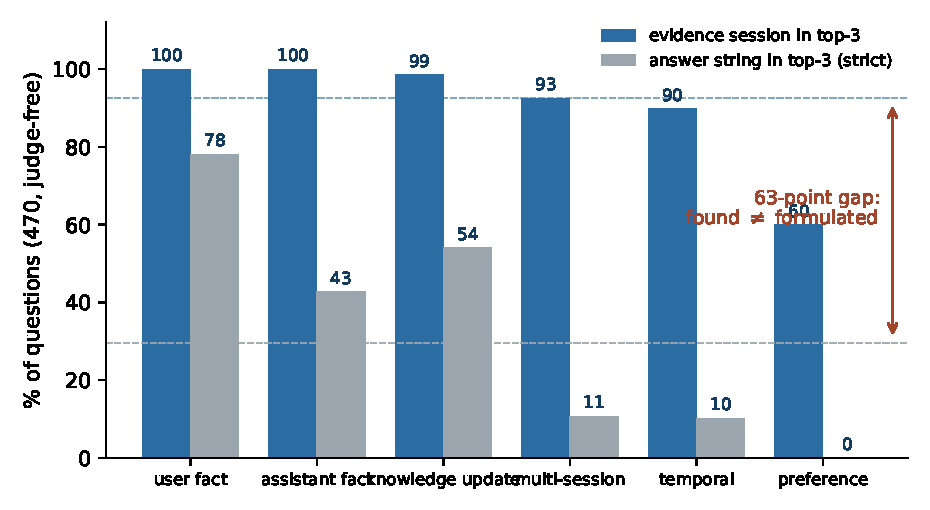
\includegraphics[width=.92\linewidth]{figs/p7fig1_gap.pdf}
\caption{Arm E on the 470 non-abstention questions, by type: the evidence session is in the top-3 for 92.6\% overall (blue), the gold answer string is present verbatim for 29.6\% (gray). The 63-point gap is the benchmark-scale face of \emph{stored is not recalled} \cite{behavior}: presence converts to surface only where the answer \emph{is} a surface (user facts), and never where formulation requires aggregation (multi-session) or computation (temporal).}
\label{fig:gap}
\end{figure}

Indexing $\sim$50 sessions and querying takes $\sim$2 seconds per question on a desktop CPU; the full benchmark runs in 17 minutes with no model loaded. Figure~\ref{fig:gap}: evidence@3 is 92.6\% overall (85.5@1, 94.5@5), with single-session types at 99--100\%, multi-session at 92.6\%, temporal at 89.8\% --- the pre-registered ordering, confirmed exactly --- and one unpredicted outlier, \emph{preference} at 60\%, which in hindsight the second law of \cite{behavior} explains: preference questions share almost no surface vocabulary with the sessions that answer them, and a lexical key has nothing to hold onto (the paraphrase boundary, met in the wild).

The strict metric tells the other half. The answer string is present in the top-3 for 78.1\% of user facts --- where the answer is a phrase the user actually typed --- but 10.7\% of multi-session and 10.2\% of temporal questions, where the gold answer (``2'', ``19 days'') exists in no session and must be \emph{computed}. Multi-session coverage sharpens the point: contrary to our registered prediction (full coverage $<30\%$ --- \textbf{refuted}), the index retrieves \emph{all} evidence sessions in the top-5 for 43.8\% of multi-session questions and at least one for another 49.6\%. The deficit is not finding the pieces; it is that nobody in this voice can add them up. \emph{Found is not formulated.}

On the 30 abstention questions the strict metric is 0\% by construction (there is nothing to find), and we note the honest limit: an extractive voice can expose absence only by returning passages a reader recognizes as off-topic; it has no way to say ``nothing''.

\section{Ingestion without the pricing tax}\label{sec:ingest}

\begin{figure}[t]
\centering
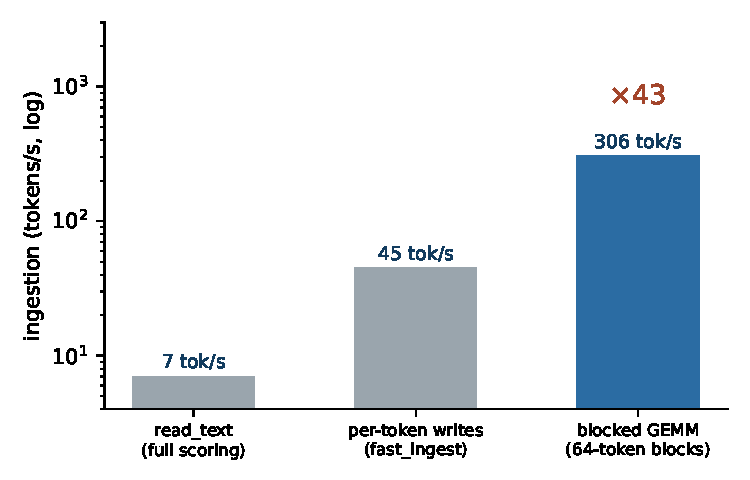
\includegraphics[width=.6\linewidth]{figs/p7fig3_ingest.pdf}
\caption{Ingestion throughput on the benchmark worker (T4 host, 2-core CPU; Qwen3-0.6B, vocab 151{,}936). The shipped read path prices the memory at every token (log-softmax, two vocabulary-sized tier readouts) and pays two rank-1 outer products per write; removing the pricing and blocking the writes into 64-token GEMMs is $\times$43. Rates from the committed \texttt{lme\_ingest\_rates.json}; the blocked figure is the median over 43 questions (min 302, max 310 tok/s).}
\label{fig:ingest}
\end{figure}

Running arm G at all was an engineering problem: the shipped read path (\texttt{read\_text}) processes $\sim$7 tokens/s on the benchmark worker, which prices a 115k-token question at over four hours. The profile is unambiguous, and worth stating because it is a design lesson: of 13.3\,ms per token (desktop CPU, Qwen3 dimensions), 11.4\,ms are the two rank-1 outer products $M \mathrel{+}= c\,q v^{\top}$ --- $\sim$50\,MB of memory traffic per token across the $4096{\times}256$ and $12288{\times}256$ matrices --- and most of the remainder is vocabulary-sized arithmetic (reported perplexity, tier readouts, score mixing) that exists to \emph{price} the memory, not to build it. The write path proper needs none of it: the gate is one scalar the frozen model already computed.

The fix has two stages, each with an exactness contract tested against the shipped path. \emph{Stage 1, write-only ingestion}: drop the pricing, keep the writes verbatim --- states are \textbf{bit-identical} to \texttt{read\_text} (all 23 state arrays, the cold store, and greedy completions; verified). \emph{Stage 2, blocked writes}: apply the outer products in 64-token blocks as one GEMM per matrix, coefficients computed against the block-start matrix, with the surprise gate batched on the GPU and the abstention reservoirs sampled one token in eight. What is exact \emph{by construction}: cold-store admissions, successor counts, surprise masses, gate statistics, token counters, aging --- none reads the matrices. What drifts, bounded and tested: trace amplitudes when the same 4-gram-and-successor repeats within one block (max $4.2\times10^{-3}$ on the validation document), the gate by float rounding ($\sim$$10^{-3}$ nats absolute on cold masses), reservoir quantiles ($1.8\%$); greedy completions on the validation state are identical to the shipped path's. The adapter stays off --- its delta rule consumes the full probability vector at every position and is inherently sequential; \cite{behavior} measured it storing no facts.

Measured end to end (Figure~\ref{fig:ingest}): 305.8 tokens/s median over the 43 questions --- 4.5M tokens ingested in 4.1 hours, rates between 302 and 310 --- against 7.05 for the shipped path: $\times$43, on the same hardware, into a behaviorally identical state. Two failed intermediate estimates (a per-token version at 45 tok/s: per-token GPU round-trips and a float64 promotion we had not priced) are preserved in the released log with their own post-mortems. The pattern repeats \cite{drafter}: the benchmark forced a capability, and the capability outlives the benchmark --- blocked ingestion ships in the tool as \texttt{read --fast}.

\section{Arm G: three voices, forty-three questions}\label{sec:armg}

\begin{figure}[t]
\centering
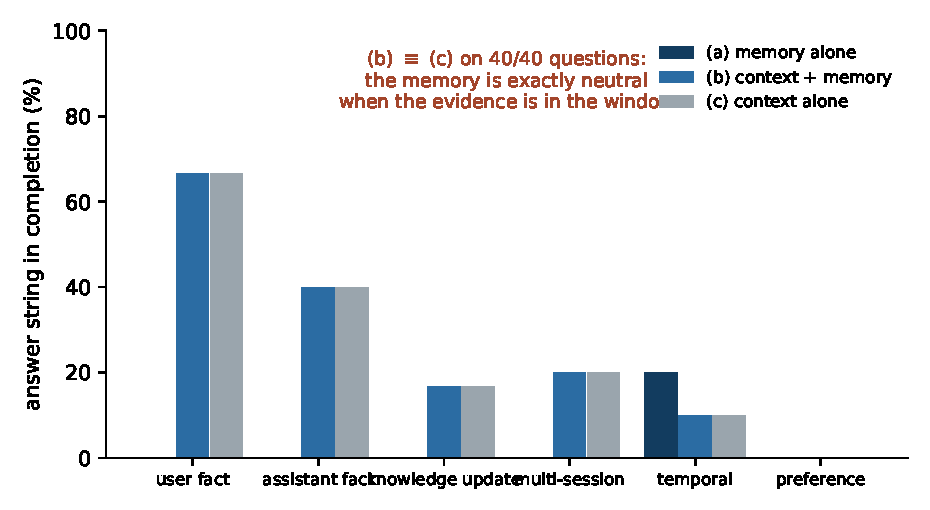
\includegraphics[width=.92\linewidth]{figs/p7fig2_voices.pdf}
\caption{Arm G (Qwen3-0.6B, containment scoring, 40 non-abstention questions): memory alone (dark) answers 5\%; the two context voices answer 25\% each --- and agree on \emph{every question}. A 121k-token memory neither helps nor hurts when the evidence is in the window: the gate prices in-window redundancy at exactly zero (law 6 of \cite{behavior}), measured here as a behavioral identity.}
\label{fig:voices}
\end{figure}

Figure~\ref{fig:voices} and the registered scorecard:

\textbf{Memory alone: 5\%} (prediction: $\leq$10\%, \textbf{confirmed}). This is the predicted negative, and the reason it was predicted matters more than the number: after 121k tokens, the state \emph{contains} the evidence (the same state's index finds it at 85\% on this subsample), but free-recall conversion needs readout trust that published settings on a cold benchmark stream do not grant \cite{behavior}, and formulation needs what \S\ref{sec:arme} showed no storage can provide. The two scored hits are both temporal-reasoning and consistent with prior luck at $n{=}24$ tokens.

\textbf{Context + memory $\equiv$ context alone: 25\% = 25\%, agreeing on 40/40 questions} (prediction: within $\pm$5 points, falsification at $-10$; \textbf{confirmed beyond its statement}). Not one question flips in either direction. The mechanism is the sixth law of \cite{behavior} doing its day job: evidence present in the window is exactly what the frozen model finds unsurprising, so the memory's scores ride along without ever changing an argmax. For deployment this is the reassuring clause: adding this memory to a RAG stack costs nothing behaviorally --- and (by \cite{drafter}) can pay for itself in speed.

\textbf{The context voices are 5$\times$ the memory voice} (prediction $\geq 4\times$, \textbf{confirmed}), and their per-type profile reproduces arm E's gradient (user facts 67\%, assistant 40\%, multi-session 20\%, temporal 10\%, preference 0\%): a 0.6B model formulates simple facts from the window and still cannot aggregate or compute --- formulation has moved from the store to the window, and hit the window's own ceiling. The three abstention questions produce no containment hit in any voice.

\section{What the laws predicted, and what refuted us}\label{sec:laws}

Eight predictions were registered across the two arms; the score is seven confirmed, one refuted.
The confirmations map one-to-one onto \cite{behavior}: the conversion wall (law 1) became the 63-point gap and the 5\% memory voice; the gate's in-window pricing (law 6) became a 40/40 behavioral identity; the paraphrase boundary (law 2) surfaced unrequested as the preference type's 60\% retrieval floor and 0\% strict score; the context-equivalence regimes (law 5) are arms (b) and (c) made external. The refutation is instructive: we predicted multi-session evidence coverage under 30\%, and measured 43.8\% full coverage --- \emph{the index finds more than we believed}. Refuted downward would have blamed retrieval; refuted upward, the burden falls squarely on formulation, which is where the laws had put it all along. We also record, per the series' habit, what did \emph{not} transfer: nothing in this benchmark tests retention or the two-occurrence rule (laws 3--4) --- every session is read once, hours before probing --- and those laws' external test remains open.

\section{Limitations}

Judge-free means leaderboard-blind: none of our metrics is comparable to LongMemEval's judged accuracy, and containment under-credits any correct but reworded answer (the preference type is entirely out of proxy). The generative arm is one small model (0.6B), one 43-question stratified sample (seed declared), one run, greedy, 24 tokens; the abstention subsample is three questions. The extractive voice is purely lexical --- its 92.6\% says as much about LongMemEval's lexical overlap between questions and evidence sessions as about the index, and both halves of that sentence are the point. Blocked ingestion's tolerances are declared and tested on a validation document, not proven in general; its reservoir subsampling delays tier activation by $\sim$4k tokens (conservative: silence). The readout-trust lever that \cite{behavior} shows unlocking conversion was deliberately \emph{not} turned here (nothing tuned on the benchmark); running the calibrated-trust protocol of \cite{drafter} on this benchmark is the designated next experiment.

\section{Conclusion}

On an external benchmark it never saw, the memory's anatomy held: the wake finds --- 92.6\% evidence retrieval at zero model cost, better coverage than its authors predicted --- and the window speaks --- every formulated answer came from context, with the memory exactly, provably neutral beside it. The gap between the two is not an engineering shortfall to hide but the very quantity the companion paper isolated on the bench: conversion, governed by trust and by the surface of keys, unchanged at benchmark scale. And as before, the benchmark paid for its passage: ingestion at $\times$43, exactness contract attached, now part of the tool. \emph{Found is not formulated} --- and knowing precisely which half your system owes you is what behavioral evaluation is for.

\appendix

\section{Reproduction}

\begingroup\emergencystretch=2.0em\hbadness=1900
Scripts (released alongside the repository, \texttt{longmemeval/}): \texttt{arm\_e\_extractive.py} (all 500 questions, CPU-only), \texttt{fast\_ingest.py} (write-only ingestion: bit-exact mode, torch-gate mode, and \texttt{fast\_ingest\_blocked}), \texttt{test\_fast\_ingest.py} (the four-state equivalence and tolerance suite), and \texttt{kaggle/} (the self-contained arm-G kernel with its clean-abort guard and pre-registration echo). Committed results: \texttt{results/lme\_arm\_e.json} (500 per-question rows and aggregates), \texttt{results/lme\_arm\_g.json} (43 rows, three voices, per-question ingestion rates), \texttt{results/lme\_ingest\_rates.json} (throughput and profile, provenance per entry). Data: LongMemEval-S from its authors' repository \cite{longmemeval}; nothing from it is redistributed here. Settings: sessions indexed as single documents (\texttt{role: content} lines); evidence@k over $k \in \{1,3,5\}$; containment after whitespace/case normalization; arm G stratified quotas $\{$temporal 10, multi-session 10, knowledge-update 6, user 6, assistant 5, preference 3$\}$ + 3 \texttt{\_abs}, seed 7 over id-sorted pools; prompts \texttt{Question:~... Answer:} with top-3 passages prepended in voices (b)/(c); greedy, $n{=}24$. Predictions, falsification thresholds, both failed sizing attempts and their post-mortems are in the released log, written before each run.\par\endgroup

\begin{thebibliography}{12}\small

\bibitem{sillage} A.~Sghairi. Sillage: Surprise-gated amplitude memory for frozen language models. Preprint, 2026. \href{https://doi.org/10.5281/zenodo.22079016}{doi:10.5281/zenodo.22079016}.

\bibitem{router} A.~Sghairi. Route the scores, not the keys: Gradient-free semantic memory for frozen language models. Preprint, 2026. \href{https://doi.org/10.5281/zenodo.22079444}{doi:10.5281/zenodo.22079444}.

\bibitem{hier} A.~Sghairi. One signal, three tiers: A routed memory hierarchy with surprise-gated consolidation. Preprint, 2026. \href{https://doi.org/10.5281/zenodo.22079471}{doi:10.5281/zenodo.22079471}.

\bibitem{fw} A.~Sghairi. Memory remembers, fast weights adapt: Two gradient-free ways to learn at test time, and why they add up. Preprint, 2026. \href{https://doi.org/10.5281/zenodo.22079481}{doi:10.5281/zenodo.22079481}.

\bibitem{drafter} A.~Sghairi. The memory pays for itself: Cross-model recall and exact speculative acceleration from one fixed-size Hebbian state. Preprint, 2026. \href{https://doi.org/10.5281/zenodo.22109220}{doi:10.5281/zenodo.22109220}.

\bibitem{behavior} A.~Sghairi. Stored is not recalled: Behavioral laws of a gradient-free memory for frozen language models. Preprint, 2026. \href{https://doi.org/10.5281/zenodo.22125859}{doi:10.5281/zenodo.22125859}.

\bibitem{longmemeval} D.~Wu, H.~Wang, W.~Yu, Y.~Zhang, K.-W.~Chang, D.~Yu. LongMemEval: Benchmarking chat assistants on long-term interactive memory. \emph{ICLR}, 2025.

\bibitem{beyondppl} X.~Song, Z.~Chen, L.~Kong, S.~Xie, X.~Dong, G.~Chen, K.~Zhang. Beyond perplexity: A behavioral evaluation framework for deployment-memory claims in LLM test-time training. arXiv:2607.00368, 2026.

\bibitem{khandelwal2020} U.~Khandelwal, O.~Levy, D.~Jurafsky, L.~Zettlemoyer, M.~Lewis. Generalization through memorization: Nearest neighbor language models. \emph{ICLR}, 2020.

\bibitem{bm25} S.~Robertson, H.~Zaragoza. The probabilistic relevance framework: BM25 and beyond. \emph{Foundations and Trends in Information Retrieval}, 3(4):333--389, 2009.

\bibitem{rag} P.~Lewis, E.~Perez, A.~Piktus, F.~Petroni, V.~Karpukhin, N.~Goyal, H.~K\"uttler, M.~Lewis, W.-t.~Yih, T.~Rockt\"aschel, S.~Riedel, D.~Kiela. Retrieval-augmented generation for knowledge-intensive NLP tasks. \emph{NeurIPS}, 2020.

\bibitem{qwen3} A.~Yang et al. Qwen3 technical report. arXiv:2505.09388, 2025.

\end{thebibliography}

\end{document}
